\vspace{-20pt}
\section{Weakly-supervised segmentation}\label{sec:sup_segmentation}

In this section we provide more qualitative examples for weakly-supervised segmentation using \gcam{} as seed for SEC (\cite{seed_eccv16}).



The last row shows 2 failure cases. In the bottom left image, the clothes of the 2 person weren't highlighted correctly. This could be because the most discriminative parts are their faces, and hence \gcam{} maps only highlights those. This results in a segmentation that only highlights the faces of the 2 people. 
In the bottom right image, the bicycles, being extremely thin aren't highlighed. This could be because the resolution of the \gcam{} maps are low ($14 \times 14$) which makes it difficult to capture thin areas.

\begin{figure*}[htp]
 \centering
 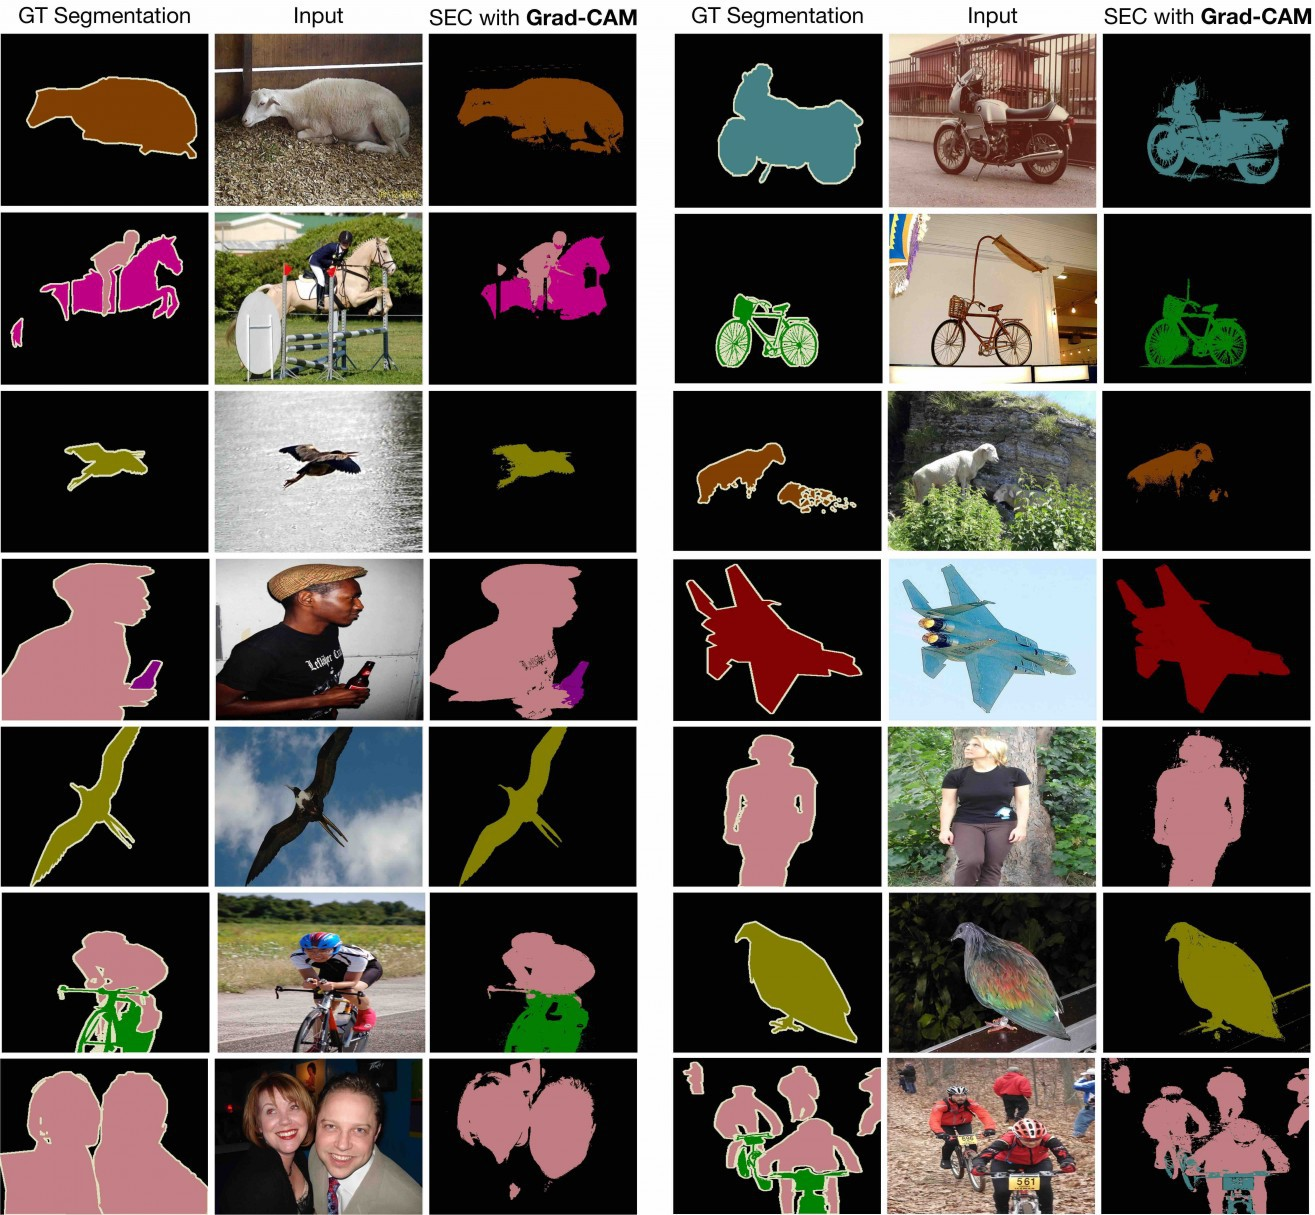
\includegraphics[width=1\linewidth]{figures/gcam_segmentation.jpg}
 \vspace{5pt}
 \caption{PASCAL VOC 2012 Segmentation results with \gcam{} as seed for SEC~\cite{seed_eccv16}.}
 \label{fig:segmentation}
\end{figure*}
